\chapter{Introduction}
\label{chap:intro}

% \epigraph{\textit{As computers have made possible the collection, storage, manipulation, and use of billions of bits of information, at quite cheap prices and through operations done at incredible speeds, ours has become the greatest data-collecting society in human history.}}{Alan F. Westin}

As \cite{westin_legal_1967} predicted in his \textit{``Legal Safeguards to Insure Privacy in a Computer Society''}, the rapid development of data surveillance technology overpowered the individual right to privacy in favour of business profit.
His postulates on privacy, written before the inventions of the internet and the Web, influenced the privacy regulations enacted in the following decades and its impact can still be seen in the European Union's (EU) General Data Protection Regulation (GDPR), through its \textit{actionable} data subject rights, which intend to give individuals the freedom to control their own personal information~\citep{westin_privacy_1967}.
Throughout his career, from 1990 to 2003, Westin also conducted a series of surveys related to consumer attitudes towards privacy, where a majority of consumers reported having \textit{``lost all control over how personal information about them is circulated and used by companies''}~\citep{kumaraguru_privacy_2005}.
Additionally, these surveys highlighted the variety of individual concerns about privacy -- the~\citeyear{westin_equifax-harris_1996}'s study showed that 25\% of the public are fundamentalists (people who are highly concerned with their privacy), 59\% pragmatists (people who are concerned with their privacy and want to protect themselves from the abuse or misuse of their personal information by companies or government agencies) and 16\% unconcerned (people who have no real concerns about privacy) and a similar study in 2003~\citep{taylor_most_2003} showed an increase in the percentage of pragmatists, 64\%, and a decrease in the unconcerned, 10\% -- a powerful reminder that, while there are more people with real concerns about the misuse of their data, different people want to have a different level of control over their privacy settings.

Following Westin's postulates, Convention 108~\citep{council_of_europe_convention_1981} was created as the first and only international data protection instrument, and over the years, enhancements have been made to address automated data processing, and trans-jurisdictional data flows.
Furthermore, in Europe, the first data protection law, the Data Protection Directive, was introduced in~\citeyear{noauthor_directive_1995} and the Charter of Fundamental Rights acknowledged the \textit{``right to the protection of personal data''} in~\citeyear{noauthor_charter_2000}.
This last one was revised and expanded in 2016 to deal with the intensive usage of digital personal data, in the form of the GDPR~\citeyearpar{noauthor_regulation_2016}.
Building on this, in 2020, and after widespread adoption of GDPR-like data protection regulations around the world~\citep{bradford_brussels_2019}, the European Commission launched its \textit{strategy for data}~\citep{european_commission_communication_2020}, with the goal of allowing the cross-sector flow of data within the EU, while ensuring that the \textit{``European rules and values, in particular personal data protection, consumer protection legislation and competition law, are fully respected''}.
Since then, we have seen the launch of a series of proposals for regulation by the European Commission and Parliament, some of them already approved and being enforced, that build on the GDPR when it comes to the processing of personal data, with the main purpose of promoting the EU's data economy while better placing EU's citizens in control of what happens to their data.
In parallel, technological development with similar goals of empowering data subjects through increased retention and control over their data has grown, however these two strands have not been well integrated to date.

\section{Thesis Overview}
\label{sec:thesis_overview}

\textcolor{blue}{ChatGPT was not used for the development of this Thesis.}

\subsection*{Part I: Introduction}

This Chapter presents the motivation of this Thesis and resulting publications, a set of definitions, as well as the projects and research stays accomplished during the Thesis.

Chapter 2 provides a state of the art on (i) decentralising the access to personal data with Solid, (ii) representing personal data processing information in a machine-readable format, and (iii) using policy languages to specify access control conditions.

Chapter 3 describes the objectives, hypotheses, assumptions, restrictions, research questions, contributions and methodology followed throughout this Thesis.

\subsection*{Part II: GDPR-Aligned Vocabularies for Personal Datastores}

Chapter 4 describes the developed vocabularies, including (i) an ODRL profile for Access Control (OAC), (ii) a metadata language for Solid (PLASMA), and (iii) rights exercising records using DPV, and includes the ontologies quality evaluation, including the detection of common pitfalls, alignment with FAIR principles and validation of competency questions with SPARQL queries.

Chapter 5 includes a legal and ethical discussion, including collaborations with the law and ethics experts in PROTECT, and other EU-funded projects, as well as with the law experts in the W3C DPVCG, and an analysis of the alignment of this Thesis with the International Organization for Standardization/International Electrotechnical Commission (ISO/IEC) 27560 standard.

\subsection*{Part III: Algorithms \& Use Cases}

Chapter 6 describes the policy matching algorithm and presents a proof of concept implementation that uses the developed vocabularies.

Chapter 7 presents the developed user interfaces and services for policy generation and metadata-keeping.

Chapter 8 presents a use case validation of this work by applying the developed resources to a health data sharing use case and as a building block for the creation of policies for the new Data Governance Act (DGA).

\subsection*{Part IV: Conclusions}

Chapter 9 describes the conclusions of this Thesis and presents future work.
\section{Motivation}
\label{sec:motivation}

GDPR~\citeyearpar{noauthor_regulation_2016} came into full effect on the 25th of May 2018 with the main objective of providing the European Union’s natural persons with the right to protection of their personal data, especially in relation to its fair, transparent, and lawful processing and sharing, including a series of rights regarding portability and erasure of data or objection to processing~\citep{ausloos_getting_2019}.
This Regulation revolves around the relationship between \textit{`data subjects'} -- the natural personal to which the personal data refers/identifies -- and \textit{`data controllers'} -- the legal entities processing said personal data.
As previously mentioned, a large part of controllers' compliance obligations are related to the data subject’s rights defined in Chapter III of the GDPR.
Information related to these rights should be provided to data subjects in a concise, transparent, comprehensible, and easily accessible manner, as well as in clear and plain language.
In particular, the so-called \textit{`Right to be informed'}, described in Articles 13 and 14, establishes the information that should be provided to the data subject at the time when the data is first collected, e.g., information on the identity of the controllers, purposes for processing, information on data transfers or existence of automated decision-making.
Moreover, data subjects should also be provided with information regarding their other rights:
the right of access to the personal data being processed;
the right of rectification of inaccurate personal data;
the right to be forgotten, i.e., the data controller has to erase the personal data requested by the subject;
the right to restrict the processing of personal data;
the right to be notified about the rectification, erasure or restriction of processing;
the right to data portability;
the right to object to any processing, including profiling;
and the right to not be subjected to automated decision-making, including profiling.

Companies usually deal with these information requirements by providing a description of their personal data-handling services in their privacy policies~\citep{linden_privacy_2020}, however, these are usually difficult to comprehend due to their complexity, lack of readability, and usage of legal terms~\citep{mcdonald_cost_2008,pasquale_black_2015,fabian_largescale_2017,lovato_more_2023}, which lead Web users to ignore them for the sake of having access to the Web services they want to use~\citep{gindin_nobody_2009,rudolph_why_2018,obar_biggest_2020}.
As such, machine-readable policy languages seem perfectly fitted to convey these information requirements in a more transparent manner -- they have been on the Web scene since the 1990s with the primary goal of establishing the conditions to access Web resources~\citep{zhao_privacy_2016,pellegrini_genealogy_2018,leicht_survey_2019}, they can offer different ways of examining privacy policies through different user interfaces~\citep{angulo_towards_2012,gerl_let_2020}, independently from the data controllers writing said policies, and they already can encode some privacy terms~\citep{cranor_platform_2002,iannella_odrl_2018}, such as the purpose for processing or recipients.
On the other hand, they are not enough to invoke specific legal terms related to the information that must be shared by data controllers, such as the legal basis for processing or the existing data subject rights.
In this context, a new wave of Semantic Web privacy and data protection vocabularies and ontologies has appeared, which can be used to represent this information, no doubt due to the proliferation of the GDPR and other data privacy-related laws~\citep{pandit_representing_2020,esteves_analysis_2022}.
Thus, such policy languages and vocabularies can be proven useful to assist data controllers in achieving GDPR alignment for their Web services and to help data subjects in the management of their rights, whether related to the transparent information requirements or their other GDPR-based rights.

More than that, the Semantic Web domain itself is of extreme importance for the representation of these privacy terms as it drives the development of open standards and specifications with interoperability and extensibility in mind.
This effort was and is being led by the World Wide Web Consortium (W3C), openly and collaboratively, with the cooperation of academia and industry.
In this context, two main lines of work are pursued:
(i) the development of common formats for data interoperability to ensure seamless integration of data from distinct sources; and 
(ii) the promotion of a structured language with the ability to document how data relates to real-world objects.
Semantic Web technologies can therefore be applied to a wide range of application fields: data integration, improved search, content management and discovery, domain modelling, or semantic annotation~\citeyearpar{noauthor_semantic_2012}.
The term \textit{`Semantic Web'} was first formulated by Sir Tim Berners-Lee, Web inventor and founder of the W3C, with the goal of having a \textit{`Web of Data'}, an extension of the Web of Documents so that data can be shared and reused in a granular manner across applications, companies and the Web community in general~\citep{berners-lee_semantic_2001}.
Solid emerged then as a natural solution to deliver this promise as a Web standards-based decentralised storage environment for data with an integrated, granular access control mechanism~\citep{sambra_solid_2016,verborgh_re-decentralizing_2022}.
Thus, such a system allows its users to choose who has access to their data and what applications to use, fulfilling GDPR's requirements of improving data portability and control for data subjects.
This implies a significant shift in the \textit{status quo} where companies gather and process data on a massive scale, constrained only by what they state in their privacy policies~\citep{nixdorf_planting_2019,robertson_excessive_2020}, where they can control what and how such information is stated.
As such, for Solid to be regarded as a tool that is fully aligned with the GDPR, the information requirements and other previously mentioned rights need to be considered and integrated into the Solid platform, in the form of user policies, notices, data access agreements, registers of users and applications, and logging of Solid-related activities.
\section{Definitions}
\label{sec:definitions}

In this Section, a series of terms, which are used throughout this Thesis, is introduced.

\subsection{Privacy terms}
\label{sec:def_privacy_terms}

The expression \textit{`privacy terms'} is usually associated with the notice that personal data handling entities use to disclose how they collect, use, store, secure, and share personal data (\ref{sec:def_personal_data}).
In this Thesis, it has a broader meaning -- the expression \textit{`privacy terms'} will be used to refer to the information that needs to be modelled to represent concepts related to the preferences and rights of data subjects and to the policies (\ref{sec:def_policies}) and obligations of data controllers regarding privacy and personal data protection~\citep{esteves_challenges_2021}.
Examples of privacy terms are the \textit{purpose} for processing personal data, the \textit{processing operation} itself, the \textit{legal basis} used by the data controller to justify the processing, or the \textit{right to data portability}.

\subsection{Policies}
\label{sec:def_policies}

Policies are documents that describe conditions for access and usage of content.
Such policies can be expressed as permissions, prohibitions, or obligations and include constraints, i.e., conditions that refine the policy rules~\citep{iannella_odrl_2018}.
In this Thesis, the focus will be on the design of policies to determine access to personal data assets stored in decentralised data systems. 
Examples of these policies are \textit{user preferences and requirements}, \textit{applications privacy policies} and \textit{data requests} or \textit{data access agreements} regarding data handling practices over personal data stored or shared through personal datastores (\ref{sec:def_pds}).

\subsection{Access control}
\label{sec:def_access_control}

The term \textit{`access control'} refers to the model used to guide the process of access to resources.
To do so, access control rules can be defined through a policy language (\ref{sec:def_policies}) with specific syntax and semantics, which are the base of a policy enforcement mechanism~\citep{cuenca_grau_access_2017}. 
Moreover, both authentication and authorisation mechanisms -- processes related to identity verification and rule-based access control enforcement, respectively -- are involved in the process of granting or denying access to resources.
In simple terms, an access control policy involves three aspects:
(i) the entity requesting/being requested access;
(ii) the requested resource(s); and 
(iii) the access rules, i.e., permissions and prohibitions on particular access modes.

\subsection{Legislation on data protection}
\label{sec:def_data_protection_law}

Before data protection was considered a fundamental right, the right to privacy emerged in 1948 through the Universal Declaration of Human Rights (UDHR) under Article 12, which stated that \textit{``No one shall be subjected to arbitrary interference with his privacy, family, home or correspondence [...]''}~\citep{united_nations_general_assembly_universal_1948}, and through the European Convention on Human Rights (ECHR) under Article 8 as \textit{``Everyone has the right to respect for his private and family life, his home and his correspondence''}~\citep{council_of_europe_european_1950}.

The first and only legally binding international instrument in the field of data protection, Convention 108~\citep{council_of_europe_convention_1981}, was created by the Council of Europe in 1981 and has been improved throughout the years to deal with automatic processing, supervisory authorities, and transborder data flows.
Following in these footsteps, the Charter of Fundamental Rights of the EU~\citeyearpar{noauthor_charter_2000}, under Article 8, acknowledged that \textit{``Everyone has the right to the protection of personal data concerning him or her''} and that \textit{``Such data must be processed fairly for specified purposes and on the basis of the consent of the person concerned or some other legitimate basis laid down by law''}, in addition to the right to privacy laid down in Article 7.
It should also be noted that in Spain, the right to privacy, or \textit{`derecho a la intimidad'}, is also a fundamental right since 1978, as defined in Article 18 of the Spanish Constitution~\citeyearpar{noauthor_constitucion_1978}.

The first EU law on data protection, the Data Protection Directive, was launched in~\citeyear{noauthor_directive_1995}.
Further legislation was enforced in 2018, to adapt the EU law on data protection to the intensive usage of digital personal data (\ref{sec:def_personal_data}) by new technological developments, in the form of the GDPR~\citeyearpar{noauthor_regulation_2016}.
In the same package, the EU launched a similar piece of legislation for the processing of personal data by state authorities for law enforcement purposes, i.e., preventing, investigating, detecting, and prosecuting criminal offences or executing criminal penalties, the Directive 2016/680~\citeyearpar{noauthor_directive_2016}.

This Thesis focuses on the requirements brought by the GDPR (\ref{sec:def_gdpr}) and also resorts to the opinions and guidelines adopted by the Article 29 Working Party, the European Data Protection Board (EDPB) and the European Data Protection Supervisor (EDPS), as well as case law and other legal literature~\citep{european_union_agency_for_fundamental_rights_and_council_of_europe_handbook_2018}.

\subsubsection{GDPR}
\label{sec:def_gdpr}

GDPR~\citeyearpar{noauthor_regulation_2016} is the landmark legislation on data protection in Europe and its effects have been felt throughout the globe, with similar pieces of regulation being discussed and adopted in American, African, and Asian countries~\citep{bradford_brussels_2019}.
It established the following principles related to the processing of personal data:
\begin{enumerate}
    \item [(i)] it should be processed in a legal, fair, and transparent manner (Article 5.1(a) on \textit{`lawfulness, fairness and transparency'}).
    \item [(ii)] the processing should be limited to the purpose specified by the data subject (Article 5.1(b) on \textit{`purpose limitation'}).
    \item [(iii)] it should include only the minimum data relevant to the purpose for which it is being processed (Article 5.1(c) on \textit{`data minimisation'}).
    \item [(iv)] the data should be accurate and possible to be corrected when necessary (Article 5.1(d) on \textit{`accuracy'}).
    \item [(v)] it should be kept only as long as it is necessary (Article 5.1(e) on \textit{`storage limitation'}).
    \item [(vi)] adequate technical and organisational measures for the security of the personal data should be ensured (Article 5.1(f) on \textit{`integrity and confidentiality'}).
    \item [(vii)] data controllers should have accountability mechanisms to demonstrate compliance with these principles (Article 5.2 on \textit{`accountability'}).
\end{enumerate}

Moreover, while analysing Chapters III and IV (\textit{`Rights of the data subject'}\footnote{\url{https://gdpr-info.eu/chapter-3/} (accessed on 15 March 2024)} and \textit{`Controller and processor'}\footnote{\url{https://gdpr-info.eu/chapter-4/} (accessed on 15 March 2024)}, respectively) of the GDPR, a set of information flows between data-related entities, i.e., data subjects, data controllers, processors and data protection officers, recipients, or supervisory authorities, can be identified.
In this context, an information flow refers to the information that has to be shared between entities so that a right or obligation can be exercised or fulfilled and GDPR's principles of lawfulness, fairness, and transparency can be respected.
As such, the following rights are provided to data subjects:

\begin{enumerate}
  \item[(Arts. 13 and 14)]\label{art:13-14} \textit{`right to be informed'} obliges data controllers to inform data subjects about any processing of personal data, whether being from data collected directly from the data subjects or other sources.
  \item[(Art. 15)]\label{art:15} \textit{`right of access'} to the personal data being processed, including a copy of the data as well as information about the purposes for processing, categories of the personal data being processed and their source, any recipients to whom the data may have been shared and corresponding measures to ensure its security, storage and retention conditions and the existence of other data subject's rights.
  \item[(Art. 16)]\label{art:16} \textit{`right to rectification'} of inaccurate or incomplete personal data.
  \item[(Art. 17)]\label{art:17} \textit{`right to be forgotten'} by the data controllers when the personal data is no longer needed for the purposes for which it was collected.
  \item[(Art. 18)]\label{art:18} \textit{`right to restriction of processing'} of personal data when its accuracy is being contested, the processing is unlawful, when the data subject needs it for any legal claims or objects to the processing.
  \item[(Art. 19)]\label{art:19} \textit{`right to be notified'} about the rectification, erasure or restriction of processing.
  \item[(Art. 20)]\label{art:20} \textit{`right to data portability'}, including the right to request that said data be transferred directly from one controller to another.
  \item[(Art. 21)]\label{art:21} \textit{`right to object'} to any processing, including profiling.
  \item[(Art. 22)]\label{art:22} \textit{`right to not be subjected to automated decision-making'}, including profiling.
\end{enumerate}
%\hyperref[art:15]{(Art. 15)} 

For instance, if a data subject wishes to exercise its \textit{`right to be forgotten'}, or \textit{`right to erasure'}, apart from raising such a request, there is the need to represent information related to the grounds on which the request is based, and the data controller needs to forward this request to other controllers which are processing the same personal data.
Figure~\ref{fig:gdpr_information_flows} shows a diagram of such information flows.
While the focus of this Thesis relies on the fulfilment of data subjects' rights, it is important to notice as well that the GDPR also contains other provisions, including obligations on data controllers and processors to maintain records of their personal data processing activities, requirements on transfers of personal data to third countries or international organisations, or on the activities of data protection supervisory authorities.

\begin{landscape}
\begin{figure}[ht]
    \centering
    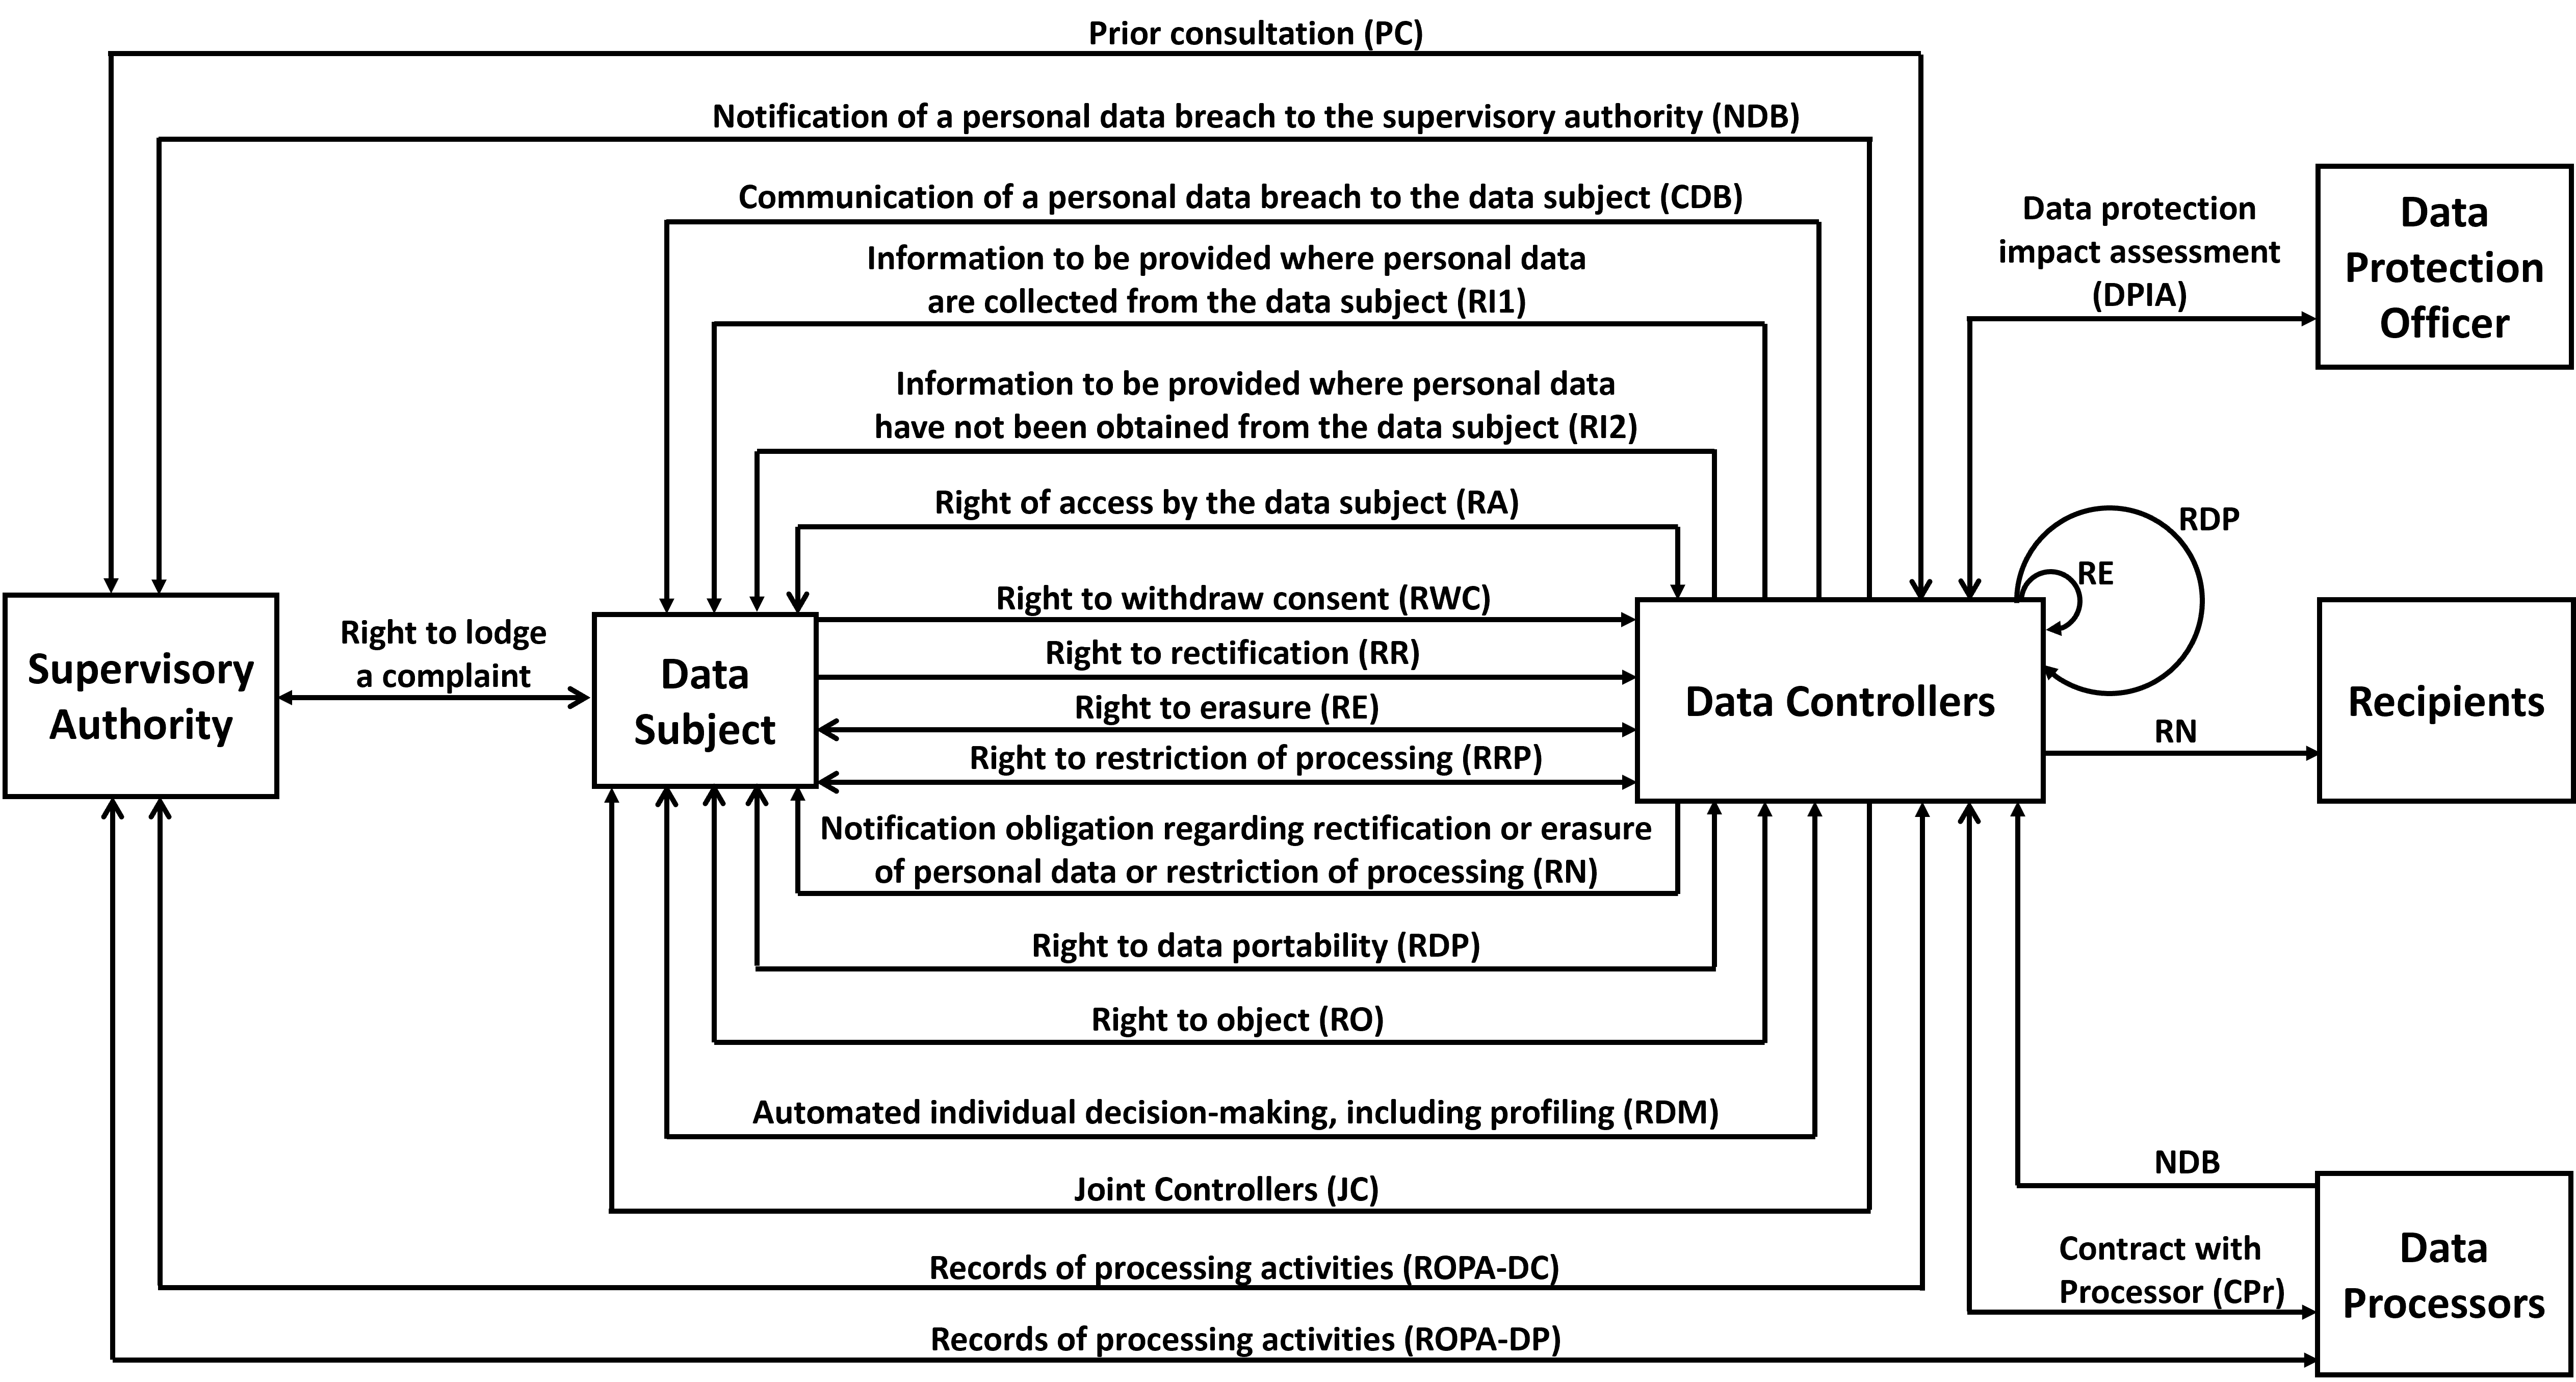
\includegraphics[width=\linewidth]{figures/chapter-1/information flow diagram.png}
    \caption[GDPR's rights and obligations as information flows.]{GDPR's rights and obligations as information flows. The bidirectional arrows represent a right or obligation in which a request for information and respective response is expected (the open arrowhead, \ding{220}, represents the entity waiting for the response, and the closed arrowhead, \ding{225}, the entity being requested). In contrast, the unidirectional arrows represent only a request or notification and no reply is expected (with the closed arrowhead, \ding{225}, representing the entity being requested or notified), adapted from~\cite{esteves_analysis_2022}.}
    \label{fig:gdpr_information_flows}
\end{figure}
\end{landscape}

\subsection{Personal data}
\label{sec:def_personal_data}

GDPR's Article 4.1~\citeyearpar{noauthor_regulation_2016} defines `personal data' as \textit{``any information relating to an identified or identifiable natural person''} such as \textit{``a name, an identification number, location data, an online identifier or to one or more factors specific to the physical, physiological, genetic, mental, economic, cultural or social identity of that natural person''}.
This Thesis relies on GDPR's definition of personal data and special categories of personal data.
In addition, it is also acknowledged that there are categories of data that are sensitive, even though they are not considered `special' under GDPR's Article 9.1, which might require additional consideration and/or protection, e.g., location data has the potential to reveal religious beliefs, sexual orientation or political opinions\footnote{DPV models \url{https://w3id.org/dpv\#SensitivePersonalData} as a subtype of \url{https://w3id.org/dpv\#PersonalData} and \url{https://w3id.org/dpv\#SpecialCategoryPersonalData} as a subtype of \url{https://w3id.org/dpv\#SensitivePersonalData}}.

Table \ref{tab:data_sensitivity}, derived from the analysis of~\cite{rumbold_what_2018}, illustrates data sensitivity for particular subcategories of data. For each data type, sensitivity is assessed from 0 to 10, i.e., from low to high sensitivity, and the relative frequency of falling into that particular sensitivity value, on a scale of 1 to 4, is also presented. For instance, data related to objects has a sensitivity of 0 and a frequency of 4 as it can not be used to identify a person, while occupation data would not be frequently classified as being highly sensitive, as demonstrated by the frequency value of 1 to the sensitivity value of 10.
In addition, data sensitivity assessment is highly contextual, as shown through the fact that the same data category can have a spectrum of sensitivity, e.g., anonymised data can have a low/high sensitivity if the risk of re-identification is very low/high, respectively. 
This evaluation of data sensitivity is also well aligned with GDPR's special categories of personal data, as can be seen through the last column of the table, where these special categories are identified and, indeed, the most sensitive are presented in Article 9, with the exception of social class data.

\begin{table}[ht]
\caption[Data sensitivity chart.]{Data sensitivity chart derived from~\cite{rumbold_what_2018}. GDPR's special categories of personal data are identified in the \textbf{GDPR} column.}
\label{tab:data_sensitivity}
\scriptsize
\centering
\begin{tabular}{|c|c||l|l|c|c|c|c|c|c|l|l|l||l|}
\multicolumn{2}{c}{} & \multicolumn{11}{c}{\textbf{DATA SENSITIVITY}} & \multicolumn{1}{c}{} \\
\hline
\multicolumn{2}{|c||}{\textbf{DATA TYPE}} & \multicolumn{1}{r|}{\cellcolor[HTML]{9A0000}{\color[HTML]{FFFFFF} 10}} & \multicolumn{1}{r|}{\cellcolor[HTML]{CB0000}{\color[HTML]{FFFFFF} 9}} & \multicolumn{1}{r|}{\cellcolor[HTML]{F56B00}{\color[HTML]{FFFFFF} 8}} & \multicolumn{1}{r|}{\cellcolor[HTML]{F8A102}7} & \multicolumn{1}{r|}{\cellcolor[HTML]{FFCB2F}6} & \multicolumn{1}{r|}{\cellcolor[HTML]{FFFE65}5} & \multicolumn{1}{r|}{\cellcolor[HTML]{D9EF8B}4} & \multicolumn{1}{r|}{\cellcolor[HTML]{A6D96A}{\color[HTML]{FFFFFF} 3}} & \multicolumn{1}{r|}{\cellcolor[HTML]{66BD63}{\color[HTML]{FFFFFF} 2}} & \multicolumn{1}{r|}{\cellcolor[HTML]{1A9850}{\color[HTML]{FFFFFF} 1}} & \multicolumn{1}{r||}{\cellcolor[HTML]{036400}{\color[HTML]{FFFFFF} 0}} & \textbf{GDPR} \\ \hline\hline
\multicolumn{1}{|c|}{} & Relating to objects & & & \multicolumn{1}{l|}{} & \multicolumn{1}{l|}{} & \multicolumn{1}{l|}{} & \multicolumn{1}{l|}{} & \multicolumn{1}{l|}{} & \multicolumn{1}{l|}{} & & & \multicolumn{1}{c||}{\cellcolor[HTML]{036400}{\color[HTML]{FFFFFF} \textbf{4}}} & \\ \cline{2-14}
\multicolumn{1}{|c|}{\multirow{-2}{*}{\textbf{\begin{tabular}[c]{@{}c@{}}Non-personal\\ data\end{tabular}}}} & \begin{tabular}[c]{@{}c@{}}Anonymised data\\ related to persons\end{tabular} & & & \cellcolor[HTML]{F56B00}{\color[HTML]{FFFFFF} \textbf{1}} & \cellcolor[HTML]{F8A102}\textbf{1} & \cellcolor[HTML]{FFCB2F}\textbf{1} & \cellcolor[HTML]{FFFE65}\textbf{1} & \cellcolor[HTML]{D9EF8B}\textbf{2} & \cellcolor[HTML]{A6D96A}{\color[HTML]{FFFFFF} \textbf{3}} & \multicolumn{1}{c|}{\cellcolor[HTML]{66BD63}{\color[HTML]{FFFFFF} \textbf{3}}} & \multicolumn{1}{c|}{\cellcolor[HTML]{1A9850}{\color[HTML]{FFFFFF} \textbf{4}}} & \multicolumn{1}{c||}{\cellcolor[HTML]{036400}{\color[HTML]{FFFFFF} \textbf{3}}} &                 \\ \hline\hline
\multicolumn{1}{|c|}{} & Opinions & & & \multicolumn{1}{l|}{} & \cellcolor[HTML]{F8A102}\textbf{3} & \cellcolor[HTML]{FFCB2F}\textbf{3} & \cellcolor[HTML]{FFFE65}\textbf{3} & \cellcolor[HTML]{D9EF8B}\textbf{3} & \cellcolor[HTML]{A6D96A}{\color[HTML]{FFFFFF} \textbf{3}} & \multicolumn{1}{c|}{\cellcolor[HTML]{66BD63}{\color[HTML]{FFFFFF} \textbf{3}}} & \multicolumn{1}{c|}{\cellcolor[HTML]{1A9850}{\color[HTML]{FFFFFF} \textbf{3}}} & & \\ \cline{2-14}
\multicolumn{1}{|c|}{} & Purchasing habits & & & \cellcolor[HTML]{F56B00}{\color[HTML]{FFFFFF} \textbf{1}} & \cellcolor[HTML]{F8A102}\textbf{2} & \cellcolor[HTML]{FFCB2F}\textbf{3} & \cellcolor[HTML]{FFFE65}\textbf{3} & \cellcolor[HTML]{D9EF8B}\textbf{3} & \cellcolor[HTML]{A6D96A}{\color[HTML]{FFFFFF} \textbf{3}} & \multicolumn{1}{c|}{\cellcolor[HTML]{66BD63}{\color[HTML]{FFFFFF} \textbf{3}}} & \multicolumn{1}{c|}{\cellcolor[HTML]{1A9850}{\color[HTML]{FFFFFF} \textbf{3}}} & & \\ \cline{2-14}
\multicolumn{1}{|c|}{} & Sex & & & \multicolumn{1}{l|}{} & \multicolumn{1}{l|}{} & \multicolumn{1}{l|}{} & \multicolumn{1}{l|}{} & \cellcolor[HTML]{D9EF8B}\textbf{3} & \cellcolor[HTML]{A6D96A}{\color[HTML]{FFFFFF} \textbf{3}} & \multicolumn{1}{c|}{\cellcolor[HTML]{66BD63}{\color[HTML]{FFFFFF} \textbf{3}}} & & & \\ \cline{2-14}
\multicolumn{1}{|c|}{} & Age & & & \multicolumn{1}{l|}{} & \cellcolor[HTML]{F8A102}\textbf{3} & \cellcolor[HTML]{FFCB2F}\textbf{3} & \cellcolor[HTML]{FFFE65}\textbf{3} & \cellcolor[HTML]{D9EF8B}\textbf{3} & \cellcolor[HTML]{A6D96A}{\color[HTML]{FFFFFF} \textbf{3}} & & & & \\ \cline{2-14}
\multicolumn{1}{|c|}{} & Income & & & \cellcolor[HTML]{F56B00}{\color[HTML]{FFFFFF} \textbf{2}} & \cellcolor[HTML]{F8A102}\textbf{3} & \cellcolor[HTML]{FFCB2F}\textbf{3} & \cellcolor[HTML]{FFFE65}\textbf{3} & \cellcolor[HTML]{D9EF8B}\textbf{3} & \cellcolor[HTML]{A6D96A}{\color[HTML]{FFFFFF} \textbf{3}} & & & & \\ \cline{2-14}
\multicolumn{1}{|c|}{} & Location & & \multicolumn{1}{c|}{\cellcolor[HTML]{CB0000}{\color[HTML]{FFFFFF} \textbf{1}}} & \cellcolor[HTML]{F56B00}{\color[HTML]{FFFFFF} \textbf{2}} & \cellcolor[HTML]{F8A102}\textbf{3} & \cellcolor[HTML]{FFCB2F}\textbf{3} & \cellcolor[HTML]{FFFE65}\textbf{3} & \cellcolor[HTML]{D9EF8B}\textbf{3} & \cellcolor[HTML]{A6D96A}{\color[HTML]{FFFFFF} \textbf{3}} & & & & \\ \cline{2-14}
\multicolumn{1}{|c|}{} & \begin{tabular}[c]{@{}c@{}}Lifestyle or\\ wellness data\end{tabular} & & \multicolumn{1}{c|}{\cellcolor[HTML]{CB0000}{\color[HTML]{FFFFFF} \textbf{3}}} & \cellcolor[HTML]{F56B00}{\color[HTML]{FFFFFF} \textbf{3}} & \cellcolor[HTML]{F8A102}\textbf{3} & \cellcolor[HTML]{FFCB2F}\textbf{3} & \cellcolor[HTML]{FFFE65}\textbf{3} & \cellcolor[HTML]{D9EF8B}\textbf{3} & \cellcolor[HTML]{A6D96A}{\color[HTML]{FFFFFF} \textbf{3}} & & & & \\ \cline{2-14}
\multicolumn{1}{|c|}{} & Occupation & \multicolumn{1}{c|}{\cellcolor[HTML]{9A0000}{\color[HTML]{FFFFFF} \textbf{1}}} & \multicolumn{1}{c|}{\cellcolor[HTML]{CB0000}{\color[HTML]{FFFFFF} \textbf{2}}} & \cellcolor[HTML]{F56B00}{\color[HTML]{FFFFFF} \textbf{3}} & \cellcolor[HTML]{F8A102}\textbf{3} & \cellcolor[HTML]{FFCB2F}\textbf{3} & \cellcolor[HTML]{FFFE65}\textbf{3} & \cellcolor[HTML]{D9EF8B}\textbf{3} & \cellcolor[HTML]{A6D96A}{\color[HTML]{FFFFFF} \textbf{3}} & & & & \\ \cline{2-14}
\multicolumn{1}{|c|}{} & Address & & & \cellcolor[HTML]{F56B00}{\color[HTML]{FFFFFF} \textbf{2}} & \cellcolor[HTML]{F8A102}\textbf{3} & \cellcolor[HTML]{FFCB2F}\textbf{3} & \cellcolor[HTML]{FFFE65}\textbf{3} & \cellcolor[HTML]{D9EF8B}\textbf{3} & \multicolumn{1}{l|}{} & & & & \\ \cline{2-14}
\multicolumn{1}{|c|}{} & Race & & & \cellcolor[HTML]{F56B00}{\color[HTML]{FFFFFF} \textbf{3}} & \cellcolor[HTML]{F8A102}\textbf{3} & \cellcolor[HTML]{FFCB2F}\textbf{3} & \cellcolor[HTML]{FFFE65}\textbf{3} & \cellcolor[HTML]{D9EF8B}\textbf{3} & \multicolumn{1}{l|}{} & & & & \textbf{Art. 9} \\ \cline{2-14}
\multicolumn{1}{|c|}{} & Ethnic group & & & \cellcolor[HTML]{F56B00}{\color[HTML]{FFFFFF} \textbf{3}} & \cellcolor[HTML]{F8A102}\textbf{3} & \cellcolor[HTML]{FFCB2F}\textbf{3} & \cellcolor[HTML]{FFFE65}\textbf{3} & \cellcolor[HTML]{D9EF8B}\textbf{3} & \multicolumn{1}{l|}{} & & & & \textbf{Art. 9} \\ \cline{2-14}
\multicolumn{1}{|c|}{} & \begin{tabular}[c]{@{}c@{}}Religious or\\ political beliefs\end{tabular} & & & \cellcolor[HTML]{F56B00}{\color[HTML]{FFFFFF} \textbf{3}} & \cellcolor[HTML]{F8A102}\textbf{3} & \cellcolor[HTML]{FFCB2F}\textbf{3} & \cellcolor[HTML]{FFFE65}\textbf{3} & \cellcolor[HTML]{D9EF8B}\textbf{3} & \multicolumn{1}{l|}{} & & & & \textbf{Art. 9} \\ \cline{2-14}
\multicolumn{1}{|c|}{} & Sexual orientation & & & \cellcolor[HTML]{F56B00}{\color[HTML]{FFFFFF} \textbf{3}} & \cellcolor[HTML]{F8A102}\textbf{3} & \cellcolor[HTML]{FFCB2F}\textbf{3} & \cellcolor[HTML]{FFFE65}\textbf{3} & \cellcolor[HTML]{D9EF8B}\textbf{3} & \multicolumn{1}{l|}{} & & & & \textbf{Art. 9} \\ \cline{2-14}
\multicolumn{1}{|c|}{} & Pregnancy & & \multicolumn{1}{c|}{\cellcolor[HTML]{CB0000}{\color[HTML]{FFFFFF} \textbf{3}}} & \cellcolor[HTML]{F56B00}{\color[HTML]{FFFFFF} \textbf{3}} & \cellcolor[HTML]{F8A102}\textbf{3} & \cellcolor[HTML]{FFCB2F}\textbf{3} & \cellcolor[HTML]{FFFE65}\textbf{3} & \cellcolor[HTML]{D9EF8B}\textbf{3} & \multicolumn{1}{l|}{} & & & & \textbf{Art. 9}  \\ \cline{2-14}
 & Transgender status & \multicolumn{1}{c|}{} & \multicolumn{1}{c|}{\cellcolor[HTML]{CB0000}{\color[HTML]{FFFFFF} \textbf{3}}} & \cellcolor[HTML]{F56B00}{\color[HTML]{FFFFFF} \textbf{3}} & \cellcolor[HTML]{F8A102}\textbf{3} & \cellcolor[HTML]{FFCB2F}\textbf{3} & \cellcolor[HTML]{FFFE65}\textbf{2} & \multicolumn{1}{l|}{} & \multicolumn{1}{l|}{} & & & & \textbf{Art. 9} \\ \cline{2-14}
\multicolumn{1}{|c|}{\multirow{-18}{*}{\textbf{\begin{tabular}[c]{@{}c@{}}Human \\ demographics, \\ behaviour,\\ thoughts \\ \& opinions\end{tabular}}}} & Social class & & & \cellcolor[HTML]{F56B00}{\color[HTML]{FFFFFF} \textbf{3}} & \cellcolor[HTML]{F8A102}\textbf{3} & \cellcolor[HTML]{FFCB2F}\textbf{3} & \multicolumn{1}{l|}{} & \multicolumn{1}{l|}{} & \multicolumn{1}{l|}{} & & & & \\ \cline{2-14} \hline\hline
\multicolumn{1}{|c|}{} & Facial images & \multicolumn{1}{c|}{} & \multicolumn{1}{c|}{} & & \cellcolor[HTML]{F8A102}\textbf{3} & \cellcolor[HTML]{FFCB2F}\textbf{3} & \cellcolor[HTML]{FFFE65}\textbf{3} & \cellcolor[HTML]{D9EF8B}\textbf{3} & \cellcolor[HTML]{A6D96A}{\color[HTML]{FFFFFF} \textbf{3}} & \multicolumn{1}{c|}{\cellcolor[HTML]{66BD63}{\color[HTML]{FFFFFF} \textbf{2}}} & & & \textbf{Art. 9} \\ \cline{2-14}
\multicolumn{1}{|c|}{} & Body images & & \multicolumn{1}{c|}{\cellcolor[HTML]{CB0000}{\color[HTML]{FFFFFF} \textbf{3}}} & \cellcolor[HTML]{F56B00}{\color[HTML]{FFFFFF} \textbf{3}} & \cellcolor[HTML]{F8A102}\textbf{3} & \cellcolor[HTML]{FFCB2F}\textbf{3} & \cellcolor[HTML]{FFFE65}\textbf{3} & \cellcolor[HTML]{D9EF8B}\textbf{3} & \cellcolor[HTML]{A6D96A}{\color[HTML]{FFFFFF} \textbf{3}} & \multicolumn{1}{c|}{\cellcolor[HTML]{66BD63}{\color[HTML]{FFFFFF} \textbf{2}}} & & & \textbf{Art. 9} \\ \cline{2-14}
\multicolumn{1}{|c|}{\multirow{-3}{*}{\textbf{\begin{tabular}[c]{@{}c@{}}Biometrics\end{tabular}}}} & \begin{tabular}[c]{@{}c@{}}Any traits processed\\ for biometrics\end{tabular} & & \multicolumn{1}{c|}{\cellcolor[HTML]{CB0000}{\color[HTML]{FFFFFF} \textbf{3}}} & \cellcolor[HTML]{F56B00}{\color[HTML]{FFFFFF} \textbf{3}} & \cellcolor[HTML]{F8A102}\textbf{3} & \multicolumn{1}{l|}{} & \multicolumn{1}{l|}{} & \multicolumn{1}{l|}{} & \multicolumn{1}{l|}{} & & & & \textbf{Art. 9} \\ \hline\hline
\multicolumn{1}{|c|}{} & Diagnoses & & \multicolumn{1}{c|}{\cellcolor[HTML]{CB0000}{\color[HTML]{FFFFFF} \textbf{3}}} & \cellcolor[HTML]{F56B00}{\color[HTML]{FFFFFF} \textbf{3}} & \cellcolor[HTML]{F8A102}\textbf{3} & \cellcolor[HTML]{FFCB2F}\textbf{3} & \multicolumn{1}{l|}{} & \multicolumn{1}{l|}{} & \multicolumn{1}{l|}{} & & & & \textbf{Art. 9} \\ \cline{2-14}
\multicolumn{1}{|c|}{} & Genetic data & \multicolumn{1}{c|}{\cellcolor[HTML]{9A0000}{\color[HTML]{FFFFFF} \textbf{3}}} & \multicolumn{1}{c|}{\cellcolor[HTML]{CB0000}{\color[HTML]{FFFFFF} \textbf{3}}} & \cellcolor[HTML]{F56B00}{\color[HTML]{FFFFFF} \textbf{4}} & \cellcolor[HTML]{F8A102}\textbf{3} & \cellcolor[HTML]{FFCB2F}\textbf{3} & \multicolumn{1}{l|}{} & \multicolumn{1}{l|}{} & \multicolumn{1}{l|}{} & & & & \textbf{Art. 9} \\ \cline{2-14}
\multicolumn{1}{|c|}{\multirow{-3}{*}{\textbf{\begin{tabular}[c]{@{}c@{}}Medical or \\ health data\end{tabular}}}} & \begin{tabular}[c]{@{}c@{}}Highly sensitive\\ diagnoses\end{tabular} & \multicolumn{1}{c|}{\cellcolor[HTML]{9A0000}{\color[HTML]{FFFFFF} \textbf{4}}} & \multicolumn{1}{c|}{\cellcolor[HTML]{CB0000}{\color[HTML]{FFFFFF} \textbf{3}}} & \multicolumn{1}{l|}{} & \multicolumn{1}{l|}{} & \multicolumn{1}{l|}{} & \multicolumn{1}{l|}{} & \multicolumn{1}{l|}{} & \multicolumn{1}{l|}{} & & & & \textbf{Art. 9} \\ \hline
\end{tabular}
\end{table}

\subsection{Decentralised data environments}
\label{sec:def_decentralised_env}

A decentralised environment for data represents a significant paradigm shift in relation to the current status of digital data management.
The Web we have today is a centralised Web where data is kept in data silos, controlled only by a handful of Big Tech players, while in a decentralised Web approach \textit{people choose where they store their data} and \textit{exert control over whom gets access to which parts of their data}~\citep{verborgh_paradigm_2017}.

Figure \ref{fig:decentralisation} illustrates the distinction between these two paradigms.
In a centralised setting, data and applications are coupled and data is kept in \textit{`walled gardens'} controlled by the entities behind centralised platforms such as Facebook, Twitter, or LinkedIn, leaving users without the possibility of reusing it elsewhere~\citeyearpar{noauthor_break_2008}.
By shifting to a decentralised Web, users are able to choose where their data is stored and are in control of their identity, while applications are detached from data, becoming \textit{``views''} over it and fostering innovation and competition through separate markets for data and services~\citep{verborgh_re-decentralizing_2022}.
Modern decentralised environments include Internet of Things (IoT) ecosystems or personal datastores (\ref{sec:def_pds}).

\begin{figure}[ht]
    \centering
    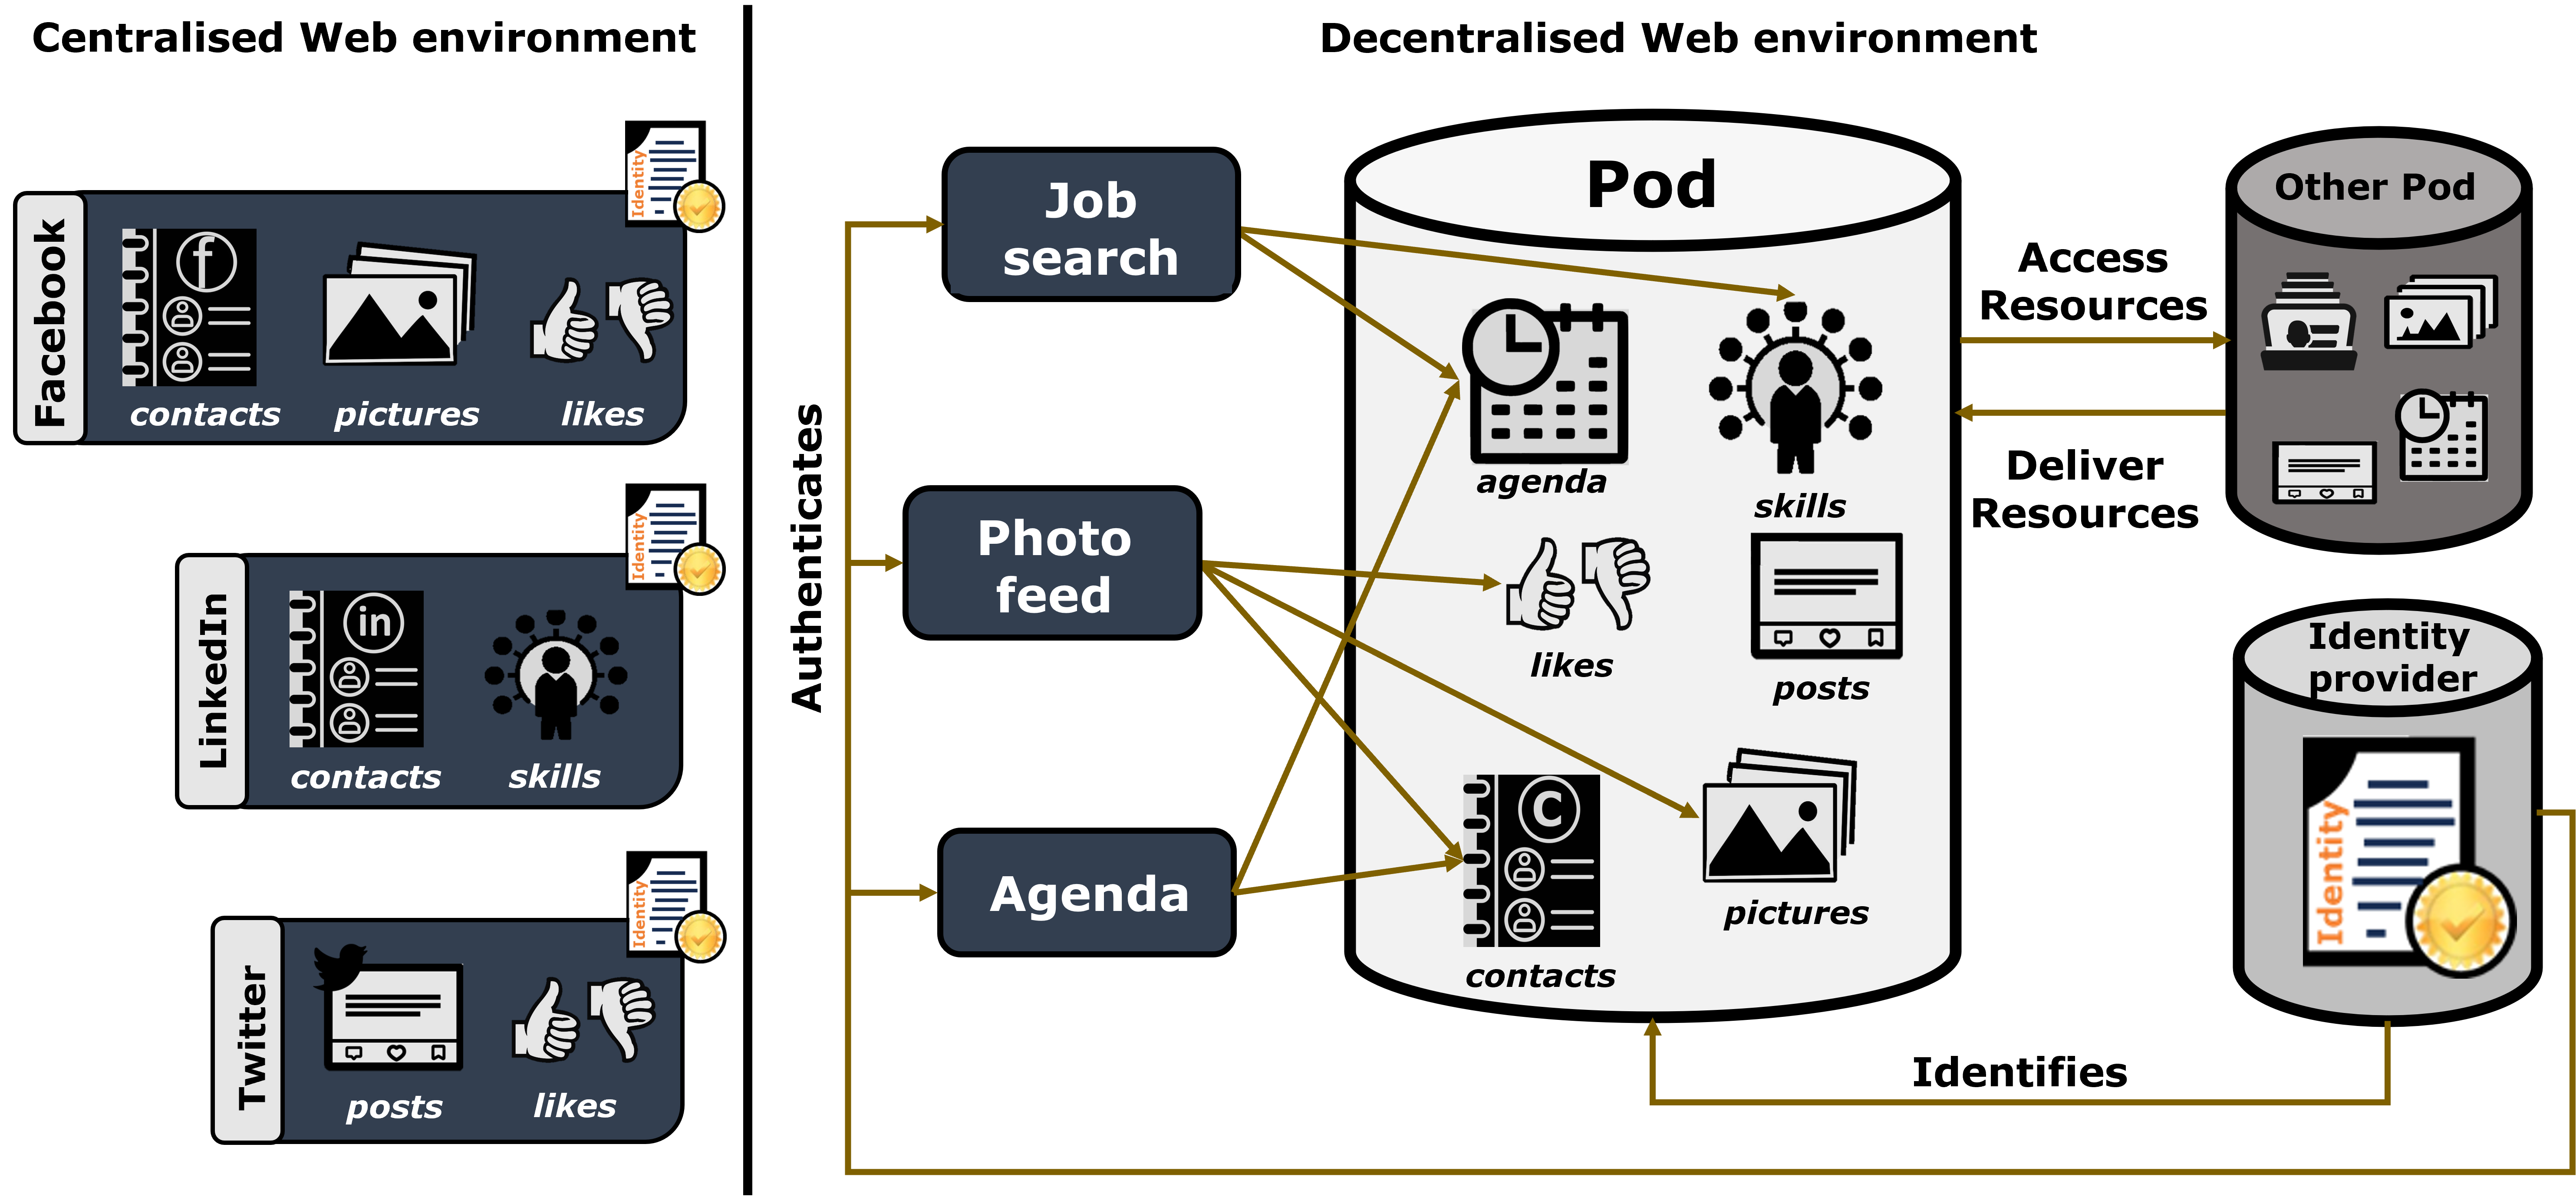
\includegraphics[width=\linewidth]{figures/chapter-1/decentralisation.png}
    \caption{Distinction between centralised and decentralised data environments.}
    \label{fig:decentralisation}
\end{figure}

This Thesis focuses on providing users with the tools to better determine access to personal data resources stored in decentralised settings, according to EU law on personal data protection.
Beyond access control (\ref{sec:def_access_control}), usage control solutions also need to be developed to provide data subjects with \textit{``control over data usage once access to the data has been granted''}~\citep{akaichi_semantic_2022}.

\subsubsection{Personal datastores}
\label{sec:def_pds}

In its \textit{TechDispatch \#3/2020}~\citep{european_data_protection_supervisor_techdispatch_2021}, the EDPS envisioned the development of personal data spaces, managed through Personal Information Management Systems (PIMS) as a mechanism to enable personal data sovereignty where \textit{``Individuals, service providers and applications would need to authenticate to access a personal storage centre''} and individuals are able to \textit{``customize what categories of data they want to share and with whom''} while keeping a record of \textit{``who has had access to their digital behaviour''} and enabling data portability and interoperability.

Such decentralised systems (\ref{sec:def_decentralised_env}) allow data subjects to directly determine who has access to their data, and under which conditions, and can actually play an important role in facilitating the exercise of data subjects’ rights, including the rights of access, erasure, and data portability or the right to withdraw consent~\citep{janssen_personal_2020}.
In the last few years, different personal datastores initiatives have been gaining prominence and adoption, including the Solid project\footnote{\url{https://solidproject.org/} (accessed on 15 March 2024)}~\citep{fallatah_personal_2023}, which is the adopted use case for the research in this Thesis.

Solid is a free, open-source initiative that delivers on the promise of decentralising the storage of data by relying on Web standards and on Semantic Web vocabularies to promote data and services interoperability. To fulfil this vision, the Solid specification relies on authentication and authorisation protocols to provide private, secure, and granular access to data stored in Solid's personal online datastores, the so-called `Pods'~\citep{mansour_demonstration_2016}.

Moreover, beyond personal datastores, decentralised initiatives at the community level are also being proposed.
For instance, data cooperative\footnote{Data infrastructure formed through the voluntary and collaborative pooling efforts of individuals.} infrastructures still give their members decision-making control over their data, while allowing them to get paid to share their data in an environment where they have more decision power than what they would have on their own or in other types of data-sharing environments~\citep{mechant_saving_2021}.
These community-level stores are also starting to be regulated, e.g., by the DGA~\citeyearpar{noauthor_regulation_2022}.
\section{Publications}
\label{sec:publications}

The following Sections list the works published and presented during the accomplishment of this Thesis. When identified with a $^{\dagger}$, the authors contributed equally to the publication work.

In addition, Figure \ref{fig:timeline} illustrates the timeline of publications, presentations, and research stays of this Thesis.

% TODO: Tas 5 in the figure -- update to start mid-2022
\begin{figure}
    \centering
    \includegraphics[width=\linewidth]{figures/chapter-1/timeline.png}
    \caption{Timeline of publications, presentations, and research stays of this Thesis.}
    \label{fig:timeline}
\end{figure}

\subsection{Journal contributions}
\label{sec:publications_journal}

\begin{enumerate}
    \item [(PJ1)] Analysis of Ontologies and Policy Languages to Represent Information Flows in GDPR. (2022) \textbf{B. Esteves}, V. Rodríguez-Doncel. \textit{Semantic Web Journal}, pp. 1--35. % TODO: update when SWJ issue is published
    \item [(PJ2)] ``Who Should I Trust with My Data?'' Ethical and Legal Challenges for Innovation in New Decentralized Data Management Technologies. (2023) H. Asgarinia$^{\dagger}$, A. Chomczyk Penedo$^{\dagger}$, \textbf{B. Esteves}$^{\dagger}$, D. Lewis. \textit{Information 14(7)}, \url{https://doi.org/10.3390/info14070351}.
    \item [(PJ3)] Is Automated Consent in Solid GDPR-Compliant? An Approach for Obtaining Valid Consent with the Solid Protocol. (2023) M. Florea$^{\dagger}$, \textbf{B. Esteves}$^{\dagger}$. \textit{Information 14(12), Special Issue on Addressing Privacy and Data Protection in New Technological Trends}, \url{https://doi.org/10.3390/info14120631}.
    \item [(PJ4)] Enhancing Data Use Ontology (DUO) for Health-Data Sharing by Extending it with ODRL and DPV. (2023) H. J. Pandit$^{\dagger}$, \textbf{B. Esteves}$^{\dagger}$.  \textit{Accepted to be published at the Semantic Web Journal}. % TODO: update when SWJ issue is published
\end{enumerate}

\subsection{Conference contributions}
\label{sec:publications_conference}

\begin{enumerate}
    \item [(PC1)] Extracting and Understanding Call-to-actions of Push-Notifications. (2022) \textbf{B. Esteves}, K. Fraser, S. Kulkarni, O. Conlan, V. Rodríguez-Doncel.  In \textit{Natural Language Processing and Information Systems. Edited by P. Rosso, V. Basile, R. Martínez, E. Métais, F. Meziane, Volume 13286}, pp. 147-–159. Springer International Publishing. \url{https://doi.org/10.1007/978-3-031-08473-7\_14}.
    \item [(PC2)] Now, Later, Never: A Study of Urgency in Mobile Push-Notifications. (2022) \textbf{B. Esteves}, K. Fraser, S. Kulkarni, O. Conlan, V. Rodríguez-Doncel. In \textit{Advances in Mobile Computing and Multimedia Intelligence. Edited by P. Delir Haghighi, I. Khalil, G. Kotsis}, pp. 38-–44. Springer Nature Switzerland. \url{https://doi.org/10.1007/978-3-031-20436-4\_4}.
    \item [(PC3)] Automating the Response to GDPR’s Right of Access. (2022) \textbf{B. Esteves}, V. Rodríguez-Doncel, R. Longares. In \textit{Legal Knowledge and Information Systems}, pp. 170–-175. IOS Press. \url{https://doi.org/10.3233/FAIA220462}.
    \item [(PC4)] Semantics for Implementing Data Reuse and Altruism Under EU’s Data Governance Act. (2023) \textbf{B. Esteves}, V. Rodríguez-Doncel,  H. J. Pandit, D. Lewis. In \textit{Knowledge Graphs: Semantics, Machine Learning, and Languages. Edited by M. Acosta et al.}, pp. 210--226. IOS Press. \url{https://doi.org/10.3233/SSW230015}.
\end{enumerate}

\subsection{Workshop contributions}
\label{sec:publications_workshop}

\begin{enumerate}
    \item [(PW1)] Challenges in the Digital Representation of Privacy Terms. (2021) \textbf{B. Esteves}. In \textit{AI Approaches to the Complexity of Legal Systems XI-XII. Edited by V. Rodríguez-Doncel, M. Palmirani, M. Araszkiewicz, P. Casanovas, U. Pagallo, G. Sartor, Volume 13048}, pp. 313–-327. Springer International Publishing. \url{https://doi.org/10.1007/978-3-030-89811-3\_22}.
    \item [(PW2)] ODRL Profile for Expressing Consent through Granular Access Control Policies in Solid. (2021) \textbf{B. Esteves}, H. J. Pandit, V. Rodríguez-Doncel. In \textit{2021 IEEE European Symposium on Security and Privacy Workshops (EuroS\&PW)}, pp. 298-–306. \url{https://doi.org/10.1109/EuroSPW54576.2021.00038}
    \item [(PW3)] Using the ODRL Profile for Access Control for Solid Pod Resource Governance. (2022) \textbf{B. Esteves}, V. Rodríguez-Doncel, H. J. Pandit, N. Mondada, P. McBennett. In \textit{The Semantic Web: ESWC 2022 Satellite Events. Edited by P. Groth, A. Rula, J. Schneider, I. Tiddi, E. Simperl, P. Alexopoulos, R. Hoekstra, M. Alam, A. Dimou, M. Tamper}, pp. 16-–20. Springer International Publishing. \url{https://doi.org/10.1007/978-3-031-11609-4\_3}
    \item [(PW4)] Semantifying the Governance of Data in Europe. (2022) \textbf{B. Esteves}, V. Rodríguez-Doncel. In \textit{18th International Conference on Semantic Systems - CEUR Workshop Proceedings, Volume 3235}. \url{https://ceur-ws.org/Vol-3235/paper17.pdf}.
    \item [(PW5)] Fostering trust with transparency in the data economy era: An integrated ethical, legal, and knowledge engineering approach. (2022) \textbf{B. Esteves}, H. Asgarinia, A. Chomczyk Penedo, B. Mutiro, D. Lewis. In \textit{Proceedings of the 1st International Workshop on Data Economy}, pp. 57-–63. \url{https://doi.org/10.1145/3565011.3569061}.
    \item [(PW6)] Towards an Architecture for Data Altruism in Solid. (2023) \textbf{B. Esteves}. In \textit{22nd International Semantic Web Conference: Posters, Demos, and Industry Tracks}. (Accepted for publication)
    \item [(PW7)] Using Patterns to Manage Governance of Solid Apps. (2023) \textbf{B. Esteves}, H. J. Pandit. In \textit{14th Workshop on Ontology Design and Patterns (WOP 2023@ISWC 2023)}. (Accepted for publication)
\end{enumerate}

\subsection{Oral presentations}
\label{sec:oral_presentations}

The following presentations were given during the realisation of this Thesis.

% TODO: create post with oral presentations with links to abstracts and slides of presentations in Zenodo}

\begin{enumerate}
    \item [(OP1)] Can privacy terms be negotiated in Solid's personal datastores? \textbf{B. Esteves}. Short talk at the \textit{2021 IEEE Symposium and Workshops on Security \& Privacy} (26/May/2021).
    \item [(OP2)] `Who should I trust with my data?': are decentralised technologies the answer to achieving ethical and lawful data governance practices? H. Asgarinia, A. Chomczyk Penedo, \textbf{B. Esteves}, D. Lewis, B. Mutiro. Presentation at the \textit{Data and the Common Workshop 2022} (04/March/2022).
    \item [(OP3)] Access control policies for Solid. \textbf{B. Esteves}. Demonstration at the \textit{2022 COST EU Workshop on Privacy Issues in Distributed Social Knowledge Graphs} (14/June/2022).
    \item [(OP4)] Establishing Data (Re-)Use Agreements Through Semantic Policies for Legally-aware Data Sharing. \textbf{B. Esteves}. Lightning talk at the \textit{SEMIC Conference 2022} (06/December/2022).
    \item [(OP5)] Altruistic (Re-)Use of Health Data through Semantic Policies. \textbf{B. Esteves}. Short talk at the \textit{2nd DPSN International Data Protection Day} (27/January/2023).
    \item [(OP6)] Privacy Receipts in Solid Pods. \textbf{B. Esteves}, J. Lindquist. Presentation at the \textit{2023 COST EU Workshop on Privacy Issues in Distributed Social Knowledge Graphs} (13/February/2023).
    \item [(OP7)] Policies in Solid: The Road Ahead. \textbf{B. Esteves}. Presentation at the \textit{Solid Symposium 2023} (31/March/2023).
    \item [(OP8)] Enhancing Solid with Legally-aware Policies. \textbf{B. Esteves}. Presentation at the \textit{Governing Artificial Intelligence International Symposium 2023} (23/May/2023).
\end{enumerate}
\section{Projects}
\label{sec:projects}

The following projects funded the work presented in this Thesis:

\paragraph{PROTECT ITN:} Protecting Personal Data Amidst Big Data Innovation (PROTECT) is an EU-funded Innovative Training Network project with the goal of developing \textit{``new ways of empowering users of digital services to understand the risks they take when they go online and to offer new ways to enable companies to incorporate data protection into digital services''} and train \textit{``a new generation of 14 early stage researchers who will integrate and apply arguments, analyses and tools from across the fields of law, ethics and knowledge engineering''}\footnote{Extracted from \url{https://cordis.europa.eu/project/id/813497} (accessed on 15 March 2024).}. This project has received funding from the European Union’s Horizon 2020 research and innovation programme under the Marie Skłodowska-Curie grant agreement No. 813497.

\paragraph{AURORA:} Achieving a new European Energy Awareness (AURORA) is an EU-funded Innovation Action project whose main objective is to \textit{``empower several thousand citizens across five locations in Denmark, England, Portugal, Slovenia, and Spain to make more informed energy decisions''}\footnote{Extracted from \url{https://cordis.europa.eu/project/id/101036418} (accessed on 15 March 2024).}. This project has received funding from the European Union’s Horizon 2020 research and innovation programme under grant agreement No. 101036418.

\paragraph{INESData:} Infraestructura para la Investigación de Espacios de Datos (INESData) is an EU-funded project with the main goal of creating and installing a data governance structure and technological components for common data spaces. This project has received funding from the European Union’s NextGenerationEU funding programme.

\paragraph{COST DKG:} COST Action on Distributed Knowledge Graphs (DKG), with grant agreement No. CA19134, whose main goal is to \textit{``create a research community for deployable Distributed Knowledge Graph technologies that are standards-based, and open, embrace the FAIR principles, allow for access control and privacy protection, and enable the decentralised publishing of high quality data''}\footnote{Extracted from \url{https://www.cost.eu/actions/CA19134/} (accessed on 15 March 2024).}.
\section{Research stays}
\label{sec:research_stays}

The research stays done in the context of this Thesis are outlined below.

\paragraph{01/10/2021 -- 01/12/2021 (2 months):} Research stay at \textit{EmPushy, Dublin, Ireland}\footnote{\url{https://www.empushy.com/} (accessed on 15 March 2024)}, supervised by Dr. Kieran Fraser. During this stay, the Annotation of Push-Notifications (APN) ontology was created to annotate push-notification datasets and train models to identify the presence of personal data in notifications' text, the intent of the notification, its persuasiveness, and so on. As this ontology is out of the scope of this Thesis, its description is omitted from this document. This work resulted in the publication of two conference papers, (PC1) and (PC2)~(\cite{esteves_extracting_2022, esteves_now_2022}, respectively). An analysis of which data to track in EmPushy's tools, and respective GDPR requirements to fulfil, was also performed with the EmPushy team. This stay was funded by the PROTECT ITN.

\paragraph{01/02/2022 -- 31/07/2022 (6 months -- half-time):} Virtual research stay at \textit{Inrupt, Inc., Boston, United States of America}\footnote{\url{https://www.inrupt.com/} (accessed on 15 March 2024)}, supervised by Pat McBennett and Nicolas Mondada. During this stay, an overview of relevant vocabularies related to the Solid ecosystem was performed. Moreover, this Thesis work on the ODRL profile for Access Control (OAC) was improved with the requirements brought by Inrupt's use cases and a Solid application (Solid ODRL access control Policies Editor -- SOPE) was developed to generate and store OAC policies in Solid Pods. This work resulted in the publication of the (PW3) workshop paper~\citep{esteves_using_2022}. This stay was funded by the PROTECT ITN.

\paragraph{01/09/2022 -- 01/12/2022 (3 months):} Research stay at \textit{ADAPT Centre, Trinity College Dublin, Dublin, Ireland}\footnote{\url{https://www.adaptcentre.ie/} (accessed on 15 March 2024)}, supervised by Prof. Dr. Harshvardhan J. Pandit and Prof. Dr. Dave Lewis. During this stay, the Policy LAnguage for Solid’s Metadata-based Access control (PLASMA) was developed. We also contributed to the development of the Data Privacy Vocabulary (DPV) specifications, including writing documentation and use cases, in particular, related to the exercising of data subjects' rights and the new DGA law. This work resulted in the publication of one conference and two workshop papers, (PC4), (PW6), and (PW7) (\cite{esteves_semantics_2023}, \cite{esteves_towards_2023} and \cite{esteves_using_2023}, respectively). This stay was funded by the PROTECT ITN.

\paragraph{01/03/2023 -- 18/03/2023 (~3 weeks):} Short-Term Scientific Mission at \textit{KNoWS, IDLab, Ghent University, Ghent, Belgium}\footnote{\url{https://knows.idlab.ugent.be/} (accessed on 15 March 2024)}, supervised by Prof. Dr. Ruben Verborgh. The main objective of this stay was to discuss and establish technical and legal requirements to align Solid with data protection principles and understand current issues and solutions that need to be dealt with and reused to implement such requirements in decentralised data-sharing environments. This mission was funded by the DKG COST Action.